\chapter{Machine Learning}
\label{ch:machine_learning}
%
This chapter will provide background on the topic of machine learning, whose role in this thesis was outlined in the introduction chapter. Our preferred definition of ``machine learning research'' was also given in that chapter, but it is worth repeating here:
%
\begin{quote}
Machine learning research seeks to develop computer systems that automatically improve their performance through experience (Mitchell et al., 1990).
\end{quote}
%	
Stated slightly differently, \emph{machine learning} is concerned with developing and analyzing algorithms used by computer systems that automatically improve their performance through experience. An earlier definition, widely attributed to Arthur Samuel, is that machine learning is ``the field of study that gives computers the ability to learn without being
explicitly programmed''\footnote{We have been unable to recover the original source of this quote. Some references cite (Samuel, 1959), but the quote is not found in reprints of this article.}. This definition also implies \emph{automatic} learning, but it suffers from the problem that the meaning of ``learn'' is not precisely defined.

As is the case in some fields, the discipline known as ``machine learning'' has drifted somewhat from its original defining aims. This will become more evident later on in this chapter when we describe the major types of machine learning problems that have developed over the past 30+ years.

The chapter is organized as follows. Section~\ref{sec:chess} presents an intuitive example of machine learning in terms of a programming task. Section~\ref{sec:modern-machine-learning} provides an overview of the modern notion of machine learning. Section~\ref{sec:supervised-learning} describes supervised learning, and finally Section~\ref{sec:unsupervised-learning} describes unsupervised learning. 

%Section~\ref{sec:semi-supervised-learning} describes semi-supervised learning, and finally Section~\ref{sec:conclusions-ml} provides concluding remarks.

\section{Computer Chess: An Example Learning Task}
\label{sec:chess}

First, by way of example, we present a classic programming task that could possibly be achieved using machine learning. The task is to create a computer program that can play chess against a human\footnote{Some of the earliest works in machine learning and artificial intelligence involved computer-playing games, such as chess and checkers. See (Turing, ????, Shannon, 1950; Samuel, 1959)}. If the task requirement were only to ``play'' chess, then the programming task would be rather trivial and would definitely not require machine learning. The programmer would simply have to encode all the rules of chess (namely how the pieces move and what happens as a result of the moves, such as captures) and then implement a random move selection function that obeys these rules. This program, undoubtedly, would be a very terrible chess player, so we add the additional requirement that the program should try to \emph{beat} a human in chess. This is now a formidable programming task, and one that has been considered by computer scientists at least as far back as Claude Shannon's 1950 paper on the subject (Shannon, 1950). Perhaps the most famous chess-playing program was initiated at Carnegie Mellon University in 1985 and later transitioned to IBM, culminating in the computer Deep Blue\textsuperscript{\textregistered} beating the chess master Garry Kasparov in a six-game match-up in 1997\footnote{We note that Kasparov has accused IBM of cheating by letting human players intervene in one of the matches.}. Nowadays, similarly advanced chess programs can run on a personal computer or even a smartphone or tablet. A full literature review of computer chess is beyond the scope of this thesis, but we refer the interested reader to (Hsu, 2002), (Spicer and Tashev, 2006), and (Russell and Norwig, 2010). Our intention in this section is to use this chess example as a way to clarify our understanding of the aim of machine learning.

\subsection{Rule-Based Methods}
\label{sec:rule-based}

Let us consider the ways in which we could go about this programming task. One way would be to extend the encoding of the rules of chess to encoding tactics and strategies of great chess masters, attempting to cover as many possible situations in chess, also known as \emph{chess positions}, as we can\footnote{We could have chosen the phrase ``contexts in chess'' rather than ``situations in chess'', thus emphasizing the conntection to context awareness, but this seems a bit awkward.}. Basically these strategy rules would instruct the computer what a chess master would do in each of the possible situations. This is essentially the approach that Deep Blue programmers took. Combined with the ability to evaluate hundreds of millions of chess positions per second, these rules eventually succeeded in beating the best human chess players.

This approach, however, hardly fits the above definition of machine learning. In fact, to create Deep Blue required many years of highly ``manual'' work of programmers refining the set of strategy rules, testing the program against human players, and repeating this process. Thus, it falls short of the aim of \emph{automatically} improving performance.

\subsection{A Trivial Chess Learning Program}
\label{sec:trivial-learning}

A trivial \emph{machine learning chess program} could work as follows: The program would simply play against itself and then at the end of the game record which side won (or whether there was a draw), as well as the set of moves in the game. Let us call one side \emph{ComputerWhite} and the other \emph{ComputerBlack}, according to convention. As the games are played, \emph{ComputerWhite} would first look-up whether the current position matches any of the records in the database and if the record corresponds to a win for \emph{ComputerWhite}, then it would play the next move listed in the record.  Otherwise, it would choose a valid move at random. \emph{ComputerBlack} would do exactly the same, and the program would continue until the game's conclusion. Another very similar version of the program would operate in the same way but allow for the other side to be played by a human. This program would not be very good when the size of the database is small, and furthermore it would learn very slowly because the records in the database would be generated by random sampling (without replacement) from the set of all possible chess games. Nonetheless, it would fit our definition of machine learning, provided that it does not require a human programmer to update the program during or after the learning process.

Such approaches are known as brute force dictionary approaches or \emph{rote learning}\footnote{Note this type of learning is similar to the so-called ``dictionary attack'' used to ``learn'' a log-in password.}. (Shannon, 1950) calculated that such a database (or dictionary) would require roughly 10\textsuperscript{43} entries. Clearly even a very efficient database containing this dictionary would require many ``Google-scale'' data warehouses, and performing look-ups in the database would be prohibitively expensive.  

It is probably fair to say that for most computing tasks, writing a trivial machine learning algorithm is fairly easy, as in the example given above. Therefore, what the discipline of machine learning is mainly concerned about is improving the learning rate and performance rate beyond that of a trivial algorithm, or ideally beyond any state-of-the-art algorithm. There are, of course, other important aspects as well, such as finding algorithms that use minimal amounts of memory or those that can produce simple/efficient models of the learned task. Learning rate and performance, however, are usually the most important aspects of a machine learning algorithm\footnote{Note that performance can be measured in different ways, a topic which we will return to in Section~\ref{sec:supervised-learning}. %TODO: I don't really talk about performance much in this section. Revisit.
In the chess example given above, a good performance metric might be the percentage of games that the computer wins against a randomly selected human player or perhaps the average \gls{fide} rating of the human players it has beaten.}. Lastly, it is important to note that there is no ``one size fits all'' machine learning algorithm. Different algorithms perform better or worse relative to their peers on different problems and learning tasks. This phenomenon has been called the ``no free lunch theorem'', and it has been shown to have a strong mathematical basis (Wolpert, 1996).

\section{Modern Machine Learning}
\label{sec:modern-machine-learning}

In this section, we describe the modern notion of machine learning, which, as we have already alluded to, has developed into something a bit different from what the early pioneers in machine learning had envisioned. That is, today there is a well-established community of machine learning researchers and practitioners whose focus is not entirely the same as what Mitchell, Samuel, or other machine learning pioneers had in mind. Our intention in pointing this out is not to denigrate the discipline of machine learning as a whole but rather to emphasize those aspects of the discipline which fall short of the original goals of machine learning. 

Let us first present a few other definitions of machine learning found in recent textbooks on the subject:

Alpaydin: ``Machine learning is programming computers to optimize a performance criterion using example data or past experience.''
Bishop: 


This definition appears quite close to that of (Mitchell et al., 1990), if we assume that ``example data'' can be generated automatically. This may be true in some cases, but in most methods described in (Alpaydin, 2010) the example data are data that have been manually labeled with the ``correct'' value relative to the performance criterion that is to be optimized. Although programs using such methods can improve their performance by obtaining more example data, if the example data cannot be generated automatically, then the method would fall short of (Mitchell et al., 1990).

Another recent definition is given by (Murphy, 2012):

Murphy: ``a set of methods that can automatically detect patterns in data, and then use the uncovered patterns to predict future data, or to perform other kinds of decision making under uncertainty (such as planning how to collect more data!).''

This definition includes the ``automatic'' aspect, similar to (Mitchell et al., 1990)

This group of methods is known as \emph{supervised learning}, and it will be discussed further in Section~\ref{sec:supervised-learning}. Similarly, many of the other methods described in (Alpaydin, 2010) are focused on discovering structure in a set of data. The ``learning task'' is to find the structure in a given set of data, but this structure is inherently dependent on the dataset itself, so this task is not a machine learning task in the sense of (Mitchell et al., 1990). Such methods fall under the category known as \emph{unsupervised learning}, which will be discussed in greater detail in Section~\ref{sec:unsupervised-learning}.

Mitchell also provides a precise definition of the concept of learning in the context of machine learning:
%
\begin{quote}
A computer program is said to \emph{learn} from experience \emph{E} with respect to some class of tasks \emph{T} and performance measure \emph{P}, if its performance at tasks in \emph{T}, as measured by \emph{P}, improves with experience \emph{E}.
\end{quote}
%
%
%

% adding economic aspects to this definition, i.e. cost of learning and value produced by tasks...?

Many learning tasks can be expressed in terms of learning a mathematical function between the inputs to the task and the desired outputs. In other words, the learning task is to find some optimal mapping between the inputs and the possible outputs. This can be expressed as follows:
%
\begin{equation}
f : \mathbf{x} \rightarrow y
\end{equation}where $f$ is a function, $\mathbf{x}$ is either a vector of inputs of arbitrary dimension, and $y \in Y=\{y_1, y_2,...y_m\}$, corresponding to the set of all possible outputs (which may or may not be finite). The function $f$ is also called a model in many textbooks on machine learning. A simple physical example function or model would be a spring scale that maps a displacement length to a weight. In this example, we know from Hooke's law that the function is linear and given by the spring constant $k$, but in many unsolved problems the form of the function is unknown, as well as its parameters. In some cases, the learning task may be framed in probabilistic terms, where the output expresses the conditional probability $p(y|\mathbf{x})$. This distribution, $p(y|\mathbf{x})$, may be intrinsically important to the application at hand, or it may be an intermediate step towards determining the most likely value of $y$ according to:
%
\begin{equation}
y = \argmax_{y \in Y} p (y|\mathbf{x})
\end{equation}
%
Machine learning techniques differ mainly in how they express and learn this unknown function $f(\mathbf{x})$ and also the form in which $y$ (and therefore the set $Y$) are expressed. For example, $Y$ may be a continuous range or a finite, discrete set. When the task involves a continuous-valued output value, it is called \emph{regression}. The spring example given above would be a regression problem. In some cases, the desired output may also be a vector of different values, representing different physical quantities (e.g. the height and weight of a person). When the output valuable is discrete, we call it \emph{classification}, since the possible values generally represent different \emph{classes} or categories. One example would be the problem of determining whether a person is male or female based on voice recordings. This example also highlights the fact that for some machine learning problems, it may be well accepted that the problem cannot be solved perfectly. Such problems may be best represented in probabilistic form.

Apart from the distinction between regression and classification, there are two main categories of machine learning techniques, based on how the unknown function $f$ is learned or approximated. The first category is known as \emph{supervised learning}. In supervised learning, a ``trainer'' supervises the learning process. The goal is essentially then to transfer the knowledge of the supervisor in the form of a mathematical or computerized model. More details on supervised learning will be covered in Section \ref{sec:supervised-learning}. The other main category is known as \emph{unsupervised learning}. In unsupervised learning, the learning process is not guided by any significant way. The goal is essentially to uncover patterns that are implicit in the data but unobvious.   More details on unsupervised learning will be covered in Section~\ref{sec:unsupervised-learning}.

From this point forward in this thesis, we will drop the distinction between the modern popular definition of machine learning and the earlier meaning of (Mitchell et al., 1990) and focus mainly on the mainstream meaning and the main techniques from machine learning. Whenever necessary, we will use the term \emph{automatic learning} to refer to the fact that improved performance takes place without requiring any human intervention.
%
\section{Supervised Learning}
\label{sec:supervised-learning}
%
As stated above, supervised learning uses a ``trainer'' to supervise the learning process. In most cases, the trainer has encoded his or her knowledge in the form of \emph{labeled data}, also known as \emph{training data} or a \emph{training set}. In terms of the function $f$ expressed above, the training consists of input-output pairs $\mathcal{D} = \{(\mathbf{x}_i, y_i)\}_{i=1}^N $, where $\mathbf{x}_i$ is an input of arbitrary dimension, $y_i$ is a ``labeled'' output, and $N$ is the number of training samples, such that $\mathcal{D}$ provides \emph{examples} of values of the function $y = f(\mathbf{x})$. In simple terms, the training data provide examples of input data that are \emph{labeled} with the correct or desired output.

It is usually the case that the training data does not exhaustively define the unknown function $f$. If, however, certain assumptions can be made about the function, then the function might be fully specified by a finite set of training data. In the simplest case, where $f$ is linear and $\mathbf{x}$ is one-dimensional, then only two training samples are needed to specify the relationship between $\mathbf{x}$ and $y$\footnote{Remember that two points define a straight line.}. Most practical examples of machine learning algorithms are more complicated due to (1) higher dimensionality, (2) non-linearity, and (3) error present in the training data.

Let us consider a simple example from the domain of context awareness. Suppose we have a smartphone application that needs to know whether the user is walking, running, or standing still (i.e. static). We refer to these as \emph{mobility contexts}. The smartphone has a GPS receiver that can record the user's position and speed, and it also has a three-axis accelerometer that can measure acceleration. In order to keep things simple, instead of using the raw accelerometer signal, we define a feature from the accelerometer data, known as \emph{dynamic acceleration}:
%
\begin{equation}
a_d = var(\{\sqrt{a_{xi}^2 + a_{yi}^2 + a_{zi}^2}\}_{i=1}^N\,)
\end{equation}
%
where $var(\cdot)$ is an operator that computes the variance over some time series of data (e.g. one second of acceleration data); $a_{xi}$, $a_{yi}$, $a_{zi}$ are the accelerations in the x, y, and z directions, respectively, for some given time epoch $i$; and $N$ is the number of samples in the time series.

A user, Mary, has painstakingly collected a dataset for developing a context-aware application and labeled whether she was walking, running, or standing still. The data are shown in Table~\ref{table:data-from-phone} below, consisting of two dimensions of input data and the labeled output. In order to keep the size reasonable, only 35 data samples are shown in the table. In Figure~\ref{fig:data-from-phone-supervised}, similar data are plotted, but now we include 1000 samples from each class.

Based on this figure, several observations can be made. We clearly see three clusters of data, corresponding to the three mobility contexts. The cluster corresponding to the ``static'' context is well separated from the other two, but in the case of the ``walking'' and ``running'' contexts, there is some overlap. Another important observation is that in the ``walking'' data, some of the values for speed are very close to 0 m/s. This could be due to errors in the data (i.e. the data from the GPS receiver might have some error) or labeling errors made by Mary. It is very common with this type of data that some labeling errors are present in the training set. For example, at the transition points between the walking and static contexts, it is difficult to accurately label which data corresponds to ``walking'' and which corresponds to ``static''\footnote{One technique to avoid such labeling errors is to remove these transition points entirely from the training set.}.

\begin{table}
\centering
\begin{tabular}{lccc}
\hline\noalign{\smallskip}
\textbf{ID} & \textbf{Speed (m/s)} & \textbf{Dyn. accel. (m\textsuperscript{2}/s\textsuperscript{4})} & \textbf{Label}\\
\hline\noalign{\smallskip}
1 & 2.56 & 21.10 & walking\\
2 & 0.94 & 28.78 & walking\\
3 & 1.24 & 31.22 & walking\\
4 & 2.99 & 36.66 & walking\\
5 & 1.24 & 36.43 & walking\\
6 & 0.64 & 29.88 & walking\\
7 & 0.73 & 34.13 & walking\\
8 & 1.68 & 28.56 & walking\\
9 & 2.72 & 32.96 & walking\\
10 & 1.82 & 38.57 & walking\\
11 & 2.10 & 30.70 & walking\\
12 & 2.80 & 49.59 & running\\
13 & 4.01 & 47.41 & running\\
14 & 3.10 & 61.96 & running\\
15 & 1.98 & 54.44 & running\\
16 & 2.33 & 53.92 & running\\
17 & 5.48 & 44.49 & running\\
18 & 4.14 & 52.38 & running\\
19 & 2.69 & 52.85 & running\\
20 & 4.73 & 44.02 & running\\
21 & 1.22 & 48.76 & running\\
22 & 4.88 & 47.78 & running\\
23 & 0.40 & 2.89 & static\\
24 & 0.92 & 0.92 & static\\
25 & 0.36 & 1.48 & static\\
26 & 1.16 & 3.37 & static\\
27 & 0.00 & 5.76 & static\\
28 & 0.28 & 3.27 & static\\
29 & 0.60 & 0.70 & static\\
30 & 0.45 & 2.97 & static\\
31 & 1.44 & 1.79 & static\\
32 & 0.11 & 1.45 & static\\
33 & 1.36 & 1.51 & static\\
34 & 1.06 & 0.03 & static\\
35 & 0.81 & 1.28 & static\\
\hline\noalign{\smallskip}
%
\end{tabular}
\caption[Example data for supervised learning]{Example data for supervised learning. The data consist of two-dimensional input data from smartphone sensors and a labelled output class.}\label{table:data-from-phone}
\end{table}
%
In this example, the goal of supervised learning would be to find a function $f$ that maps the input data $(speed^i,a_d^i)$ to the correct output class, i.e.  $\{`walking\textrm',$ $`running\textrm',`static\textrm'\}$, such that the number of errors are minimized. In this context, errors could be defined as input data that are mapped to the wrong output class, also known as misclassifications.
%
\begin{figure}

\begin{center}
    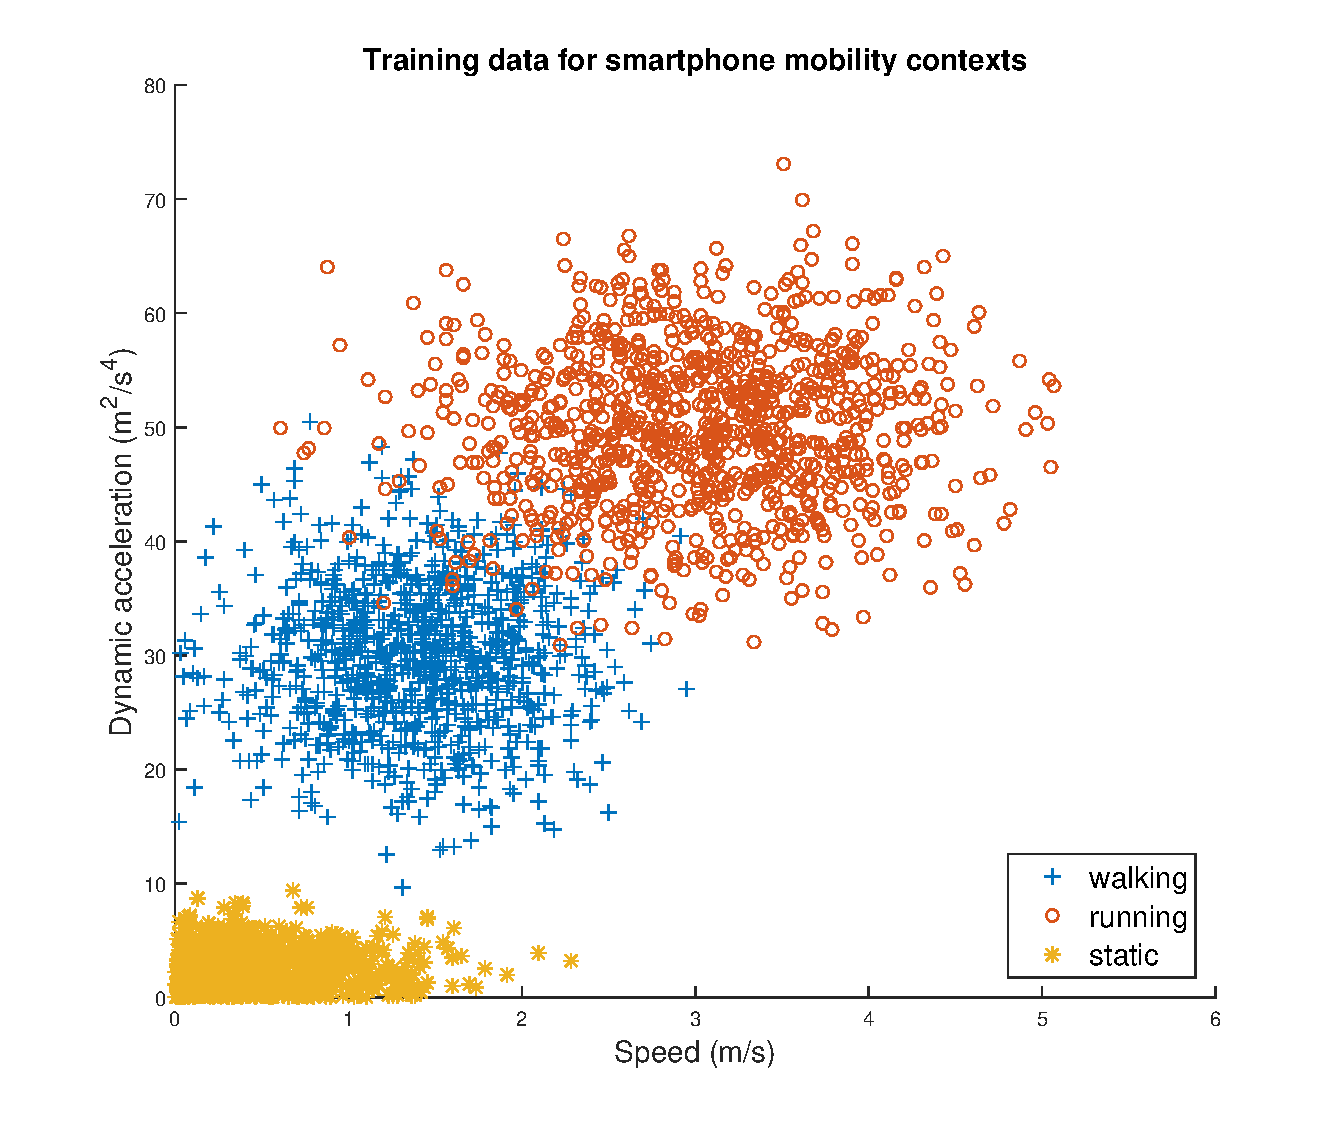
\includegraphics[width=1.0\textwidth]{Images/figChapter3-1}
  \end{center}
  \caption[Training data for supervised learning]{Example training data for supervised learning. The data are similar to those shown in Table~\ref{table:data-from-phone}. Note the partial overlap between the ``walking'' and ``running'' classes.}
  \label{fig:data-from-phone-supervised}
\end{figure}

Three important interrelated concepts should now be introduced: \emph{generalization}, \emph{underfitting}, and \emph{overfitting}. Generalization refers to the idea that supervised learning should ``generalize'' beyond the specific examples given in the training set. In other words, the goal is not simply to map the inputs to the outputs for the given training set but rather to find a mapping function that works well on some yet unseen data. If the goal were simply to fit a function to the training set, then it would be trivial to write a function that performs with zero errors (e.g. a simple lookup table would do the job).

%Ideally the function should cover the entire input space.

Overfitting refers to the situation where the supervised learning algorithm has produced a mapping function that follows the training data in too much detail. Keep in mind that every training set is somehow incomplete and imperfect. If the training results in a function that does not properly take into account the gaps and the noise in the training data, then it will \emph{overfit} the training data and will not generalize well. It is also possible that a mapping function \emph{underfits} the training data. This usually means that the mapping function is overly simple, for example, using a linear model for data that is inherently non-linear. Therefore, good generalization lies in between the two extremes of underfitting and overfitting. The goal of learning is more precisely defined as minimizing the \emph{generalization error}, which is the average error rate that will be produced by any future data, and this means finding a model that neither overfits nor underfits. Of course, it is difficult to estimate the true generalization error. The most common approach is to use an independent \emph{test set}. A test set is simply another labeled dataset that is not used in the learning process but is reserved for measuring the generalization error after learning has already taken place.

A test set provides a way to measure the generalization error and see whether any overfitting or underfitting is occurring, but the question remains: How does one determine the right type of function or model to fit to the training data? This process is known as \emph{model selection}. In model selection, we siphon off yet another portion from the training set, known as the \emph{validation set}. The model selection process then proceeds as follows:
%
\begin{enumerate}
\item Choose a hypothesis set $\mathpzc{H}$ containing different hypothesis function types to be used in model selection. This hypothesis set can be of one particular function class, such as the set of all linear functions or can be of several different classes. The goal is to include within the hypothesis set a class of functions that match well with the underlying data under investigation. This is , however, non-trivial and may require some precursory \emph{data exploration}.
%
\item Given the hypothesis set $\mathpzc{H}$, for each hypothesis class $\mathpzc{H}_i \in \mathpzc{H}$, use the training set $\mathcal{D}$ to find the best function $h_i \in \mathpzc{H_i}$.  For example, if $\mathpzc{H}_i$ is the set of all linear functions of the form $h(x) = a * x + b$, then this step is equivalent to finding the parameters $a$ and $b$ that best match the training data, according to some linear regression estimator, e.g. the least squares estimator.
%
\item Now we have a set of fitted functions ${h_i} \in \mathpzc{H}$, and the next step is to choose the best one. For this, we use the validation set to measure the error rate and choose the function with the lowest error, which we denote $h_{best}$, and its hypothesis class is denoted by $\mathpzc{H}_{best}$.

\item Finally, fit a new function $h_i \in \mathpzc{H}_{best}$ using the training set plus the validation set, and measure its  error using the test set. Since the test set was not used in the learning process, the resulting error rate can be considered an estimate of the generalization error.
\end{enumerate}
%
Depending on the amount of labeled data available, and the complexity of the underlying structure in the data, it may be necessary to repeat this process with different divisions of the labeled data into the respective training set, validation set, and  set. The standard technique for this repetition process is known as \emph{cross-validation}. Due to space limitations, we will not cover cross-validation in detail, but it was employed in [P3] and [P4].%TODO.
%
\section{Unsupervised Learning}
\label{sec:unsupervised-learning}
Unsupervised learning is, in many ways, quite similar to supervised learning, except that there are no labeled data. In other words, there are only input data, and the goal is to learn something about the structure or patterns in the input data. In this way, unsupervised learning is very similar to traditional statistical methods, where the goal is to infer a statistical model from a set of data. Many unsupervised learning methods, such as density estimation, come straight from statistics. Others differ only in the name or some other superficial characteristics. Especially in recent years, there are large overlaps between statistics research and unsupervised learning research\footnote{This is also true to a certain extent in supervised learning, but the similarity is more striking in unsupervised learning.}.

\begin{figure}
  \begin{center}
    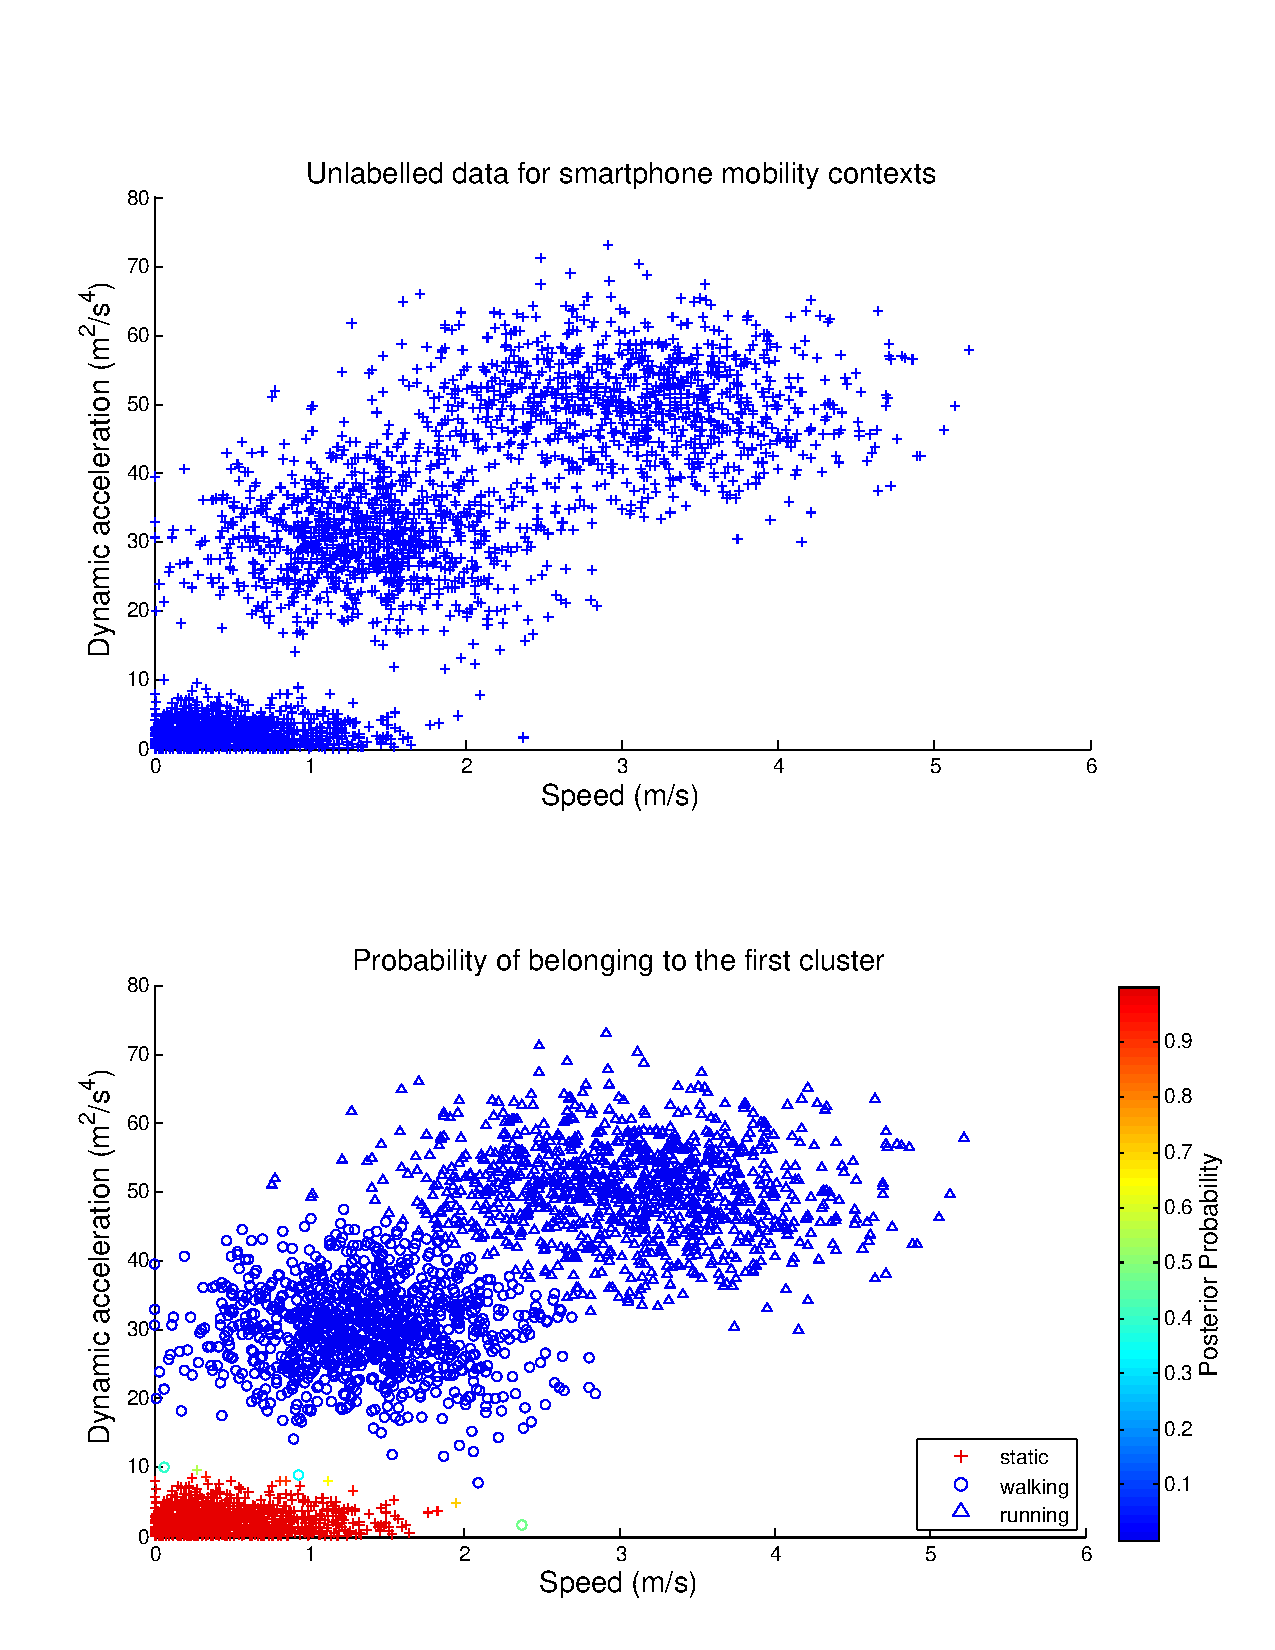
\includegraphics[width=1.0\textwidth]{Images/figChapter3-2}
  \end{center}
  \caption[Input data for unsupervised learning and one clustering result]{The top plot shows example input data for unsupervised learning. In contrast to Figure~\ref{fig:data-from-phone-supervised} no labels are available. The bottom plot shows one result from the EM-based clustering. The color of the points shows the posterior probability that the points belong to the first component in a GMM. Data labels are shown strictly for demonstration purposes. In a real situation, no such label would be available to interpret the unsupervised learning result.}
  \label{fig:data-from-phone-unsupervised}
\end{figure}

Consider again the data presented in Table~\ref{table:data-from-phone} and Figure~\ref{fig:data-from-phone-supervised}. Suppose Mary had not gone to the trouble of labeling the data with the actual mobility context associated with each data sample. We would have then only a two-dimensional dataset of input data, and we could make a similar plot as Figure~\ref{fig:data-from-phone-supervised}, except the legend would be missing and we would also not have the information necessary to label the samples with different colors as in Figure~\ref{fig:data-from-phone-supervised}. The top part of Figure~\ref{fig:data-from-phone-unsupervised} shows such a plot.
%

One unsupervised learning task would be identify different clusters or groups present in the data. Depending on the data and the application, it may or may not be apparent how many clusters are inherently present in the data, so the number of clusters may also be a parameter to determine as part of the unsupervised learning task. As is the case in supervised learning, there are a plethora of different unsupervised learning algorithms available in the literature that perform clustering. Possibilities include k-means clustering (Hartigan and Wong, 1979), \acrshort{optics} (Ankherst et al., 1999), and the \gls{em} algorithm (Dempster et al., 1977). In particular, the EM algorithm has its roots in statistitcs and can fit observed data to an arbitrary statistical model.

To provide an example of clustering, we used the EM algorithm to fit a \gls{gmm} to the data that we have previously seen in the top half of Figure~\ref{fig:data-from-phone-unsupervised}. A GMM is of the form:
%
\begin{equation}
 p(\mathbf{x}|\Theta) = \sum\limits_{k=1}^K \pi_k \phi_k(\mathbf{x}; \boldsymbol{\theta}_k)
\end{equation}
%
where $\mathbf{x}$ is a random vector, $K$ is the number of components in the mixture model, $\phi_k(\mathbf{x}; \boldsymbol{\theta}_k)$ are normal distributions with parameters $\boldsymbol{\theta}_k = (\boldsymbol{\mu_k}, \mathbf{\Sigma_k})$, $\pi_k$ are mixing weights satisfying $\pi_1 + ... + \pi_K = 1, \pi_k \geq 0$, and $\Theta = \{\pi_1,...,\pi_K,\theta_1, ..., \theta_K\}$ is the complete set of model parameters\footnote{The notation used for the GMM is similar but not identical to that given in (Bilmes, 1998).}.

The EM algorithm itself is a widely-used iterative algorithm used to find the \gls{mle} of the model parameters (which we denote with $\Theta$ as above) for an underlying distribution $p(\mathbf{x}|\Theta)$ used to model a given dataset, which we denote as $\mathcal{D} = (\mathbf{x}_1,..., \mathbf{x}_N)$ (Bilmes, 1998). The MLE is obtained by maximizing a function $Q$ equal to the expected value of the loglikelihood $\mathcal{L}(\Theta|\mathcal{D},\mathcal{Y})$, given the observed data $\mathcal{D}$ and the current parameter estimates $\Theta^{(i-1)}$:
%
\begin{gather}
  Q(\Theta,\Theta^{(i-1)}) = E[\log \mathcal{L}(\Theta|\mathcal{D}, \mathcal{Y})|\mathcal{D},\Theta^{(i-1)})]
     = E[\log p(\mathcal{D}, \mathcal{Y}|\Theta)|\mathcal{D},\Theta^{(i-1)})]
\end{gather}
%
where $\mathcal{Y} = (y_1, ..., y_N)$ is a vector of latent variables that indicate to which component of the GMM a given data sample $\mathbf{x}_j$ belongs. The latent variables can be expressed in various ways, but perhaps the simplest expression is that $y_j = k$ when $\mathbf{x}_j$ belongs to component $k$. In the above equation $i$ indexes the current iteration interval of the algorithm, so $\Theta^{(i-1)}$ represents the parameter estimate from the previous iteration (or the initial estimate, if $i=1$).

Before applying the EM algorithm to find the parameters $\Theta$ of a GMM, one must decide on the number of components $K$ to incorporate into the GMM. As we shall see, each component $k$ in the model will correspond to a cluster in the final clustering result; thus, this step is, in practice, the same as determining the number of clusters, and we can consider $K$ to be a hyperparameter in the estimation problem.

Various methods can be used to determine the best value for $K$. For low-dimensional data, a practical method is to simply plot the data (as we did in the top half of Figure~\ref{fig:data-from-phone-unsupervised}) and try to visualize the inherent number of clusters. For high-dimensional data ($D>3$), this simple approach is not necessarily adequate, nor does it support the goal of automation described earlier. Therefore, a more sophisticated, systematic approach may be preferred, such as the one described in (Vlassis and Likas, 2002). For this example, we assume in the interest of space that the choice of $K$ is already clear, and for these data $K=3$ seems to be a reasonable choice.

The next step is simply to apply the EM algorithm to determine the parameters $\Theta$ of our three-component GMM. A detailed description of the EM algorithm is beyond the scope of this thesis, but here we provide a brief overview.

First, EM requires an initial estimate of $\Theta$, and various initialization techniques to provide sensible initial estimates can be found in the literature . A simple approach is to use the given dataset $\mathcal{D}$: e.g. select $K$ random samples to initialize $\boldsymbol{\mu_k}$ and use the covariance matrix of $\mathcal{D}$ for each of the initial $K$ covariance matrices $\Sigma_k$ (Smyth, 2015).

After initialization, the algorithm then alternates between computing an expectation function (known as the E-step) and finding the parameters $\Theta$ that maximize this function (known as the M-step). At each E-step, the algorithm calculates a new $Q(\Theta,\Theta^{(i-1)})$. In the M-step, an updated estimate $\Theta^{(i)}$ of the parameter set is obtained by maximizing $Q(\Theta,\Theta^{(i-1)})$, according to:
%
\begin{equation}
 \Theta^{(i)} = \argmax_\Theta{Q(\Theta,\Theta^{(i-1)})}
\end{equation}
%
The algorithm terminates when $Q(\Theta,\Theta^{(i-1)})$, evaluated at $\Theta$ = $\Theta^{(i)}$, converges towards a maximum value (i.e. improvement is below some threshold value $\epsilon$).

Finally, once the parameters $\Theta$ are estimated, we can determine the posterior probability that a data sample $\mathbf{x}_j$ belongs to a particular component $k$ of the GMM, according to its so-called ``membership weight'' (Smyth, 2015):
%
\begin{equation}
  w_j^k = p(y_j = k|\mathbf{x}_j, \Theta) =  \frac{p_k(\mathbf{x}_j|\theta_k) \pi_k}{ \sum_{m=1}^K p_m(\mathbf{x}_j|\theta_m) \pi_m }
\end{equation}
%
Recall that each component of the GMM corresponds to a cluster, and therefore the membership weight for a given $k$ is the posterior probability that the data sample belongs to cluster $k$. The bottom half of Figure~\ref{fig:data-from-phone-unsupervised} and Figure~\ref{fig:data-from-phone-unsupervised2} show the posterior probabilities for our example data, corresponding to membership in each of the three clusters. Note that a dividing line between membership in each cluster can be drawn where the posterior probability reaches 0.5.
%
\begin{figure}
  \begin{center}
    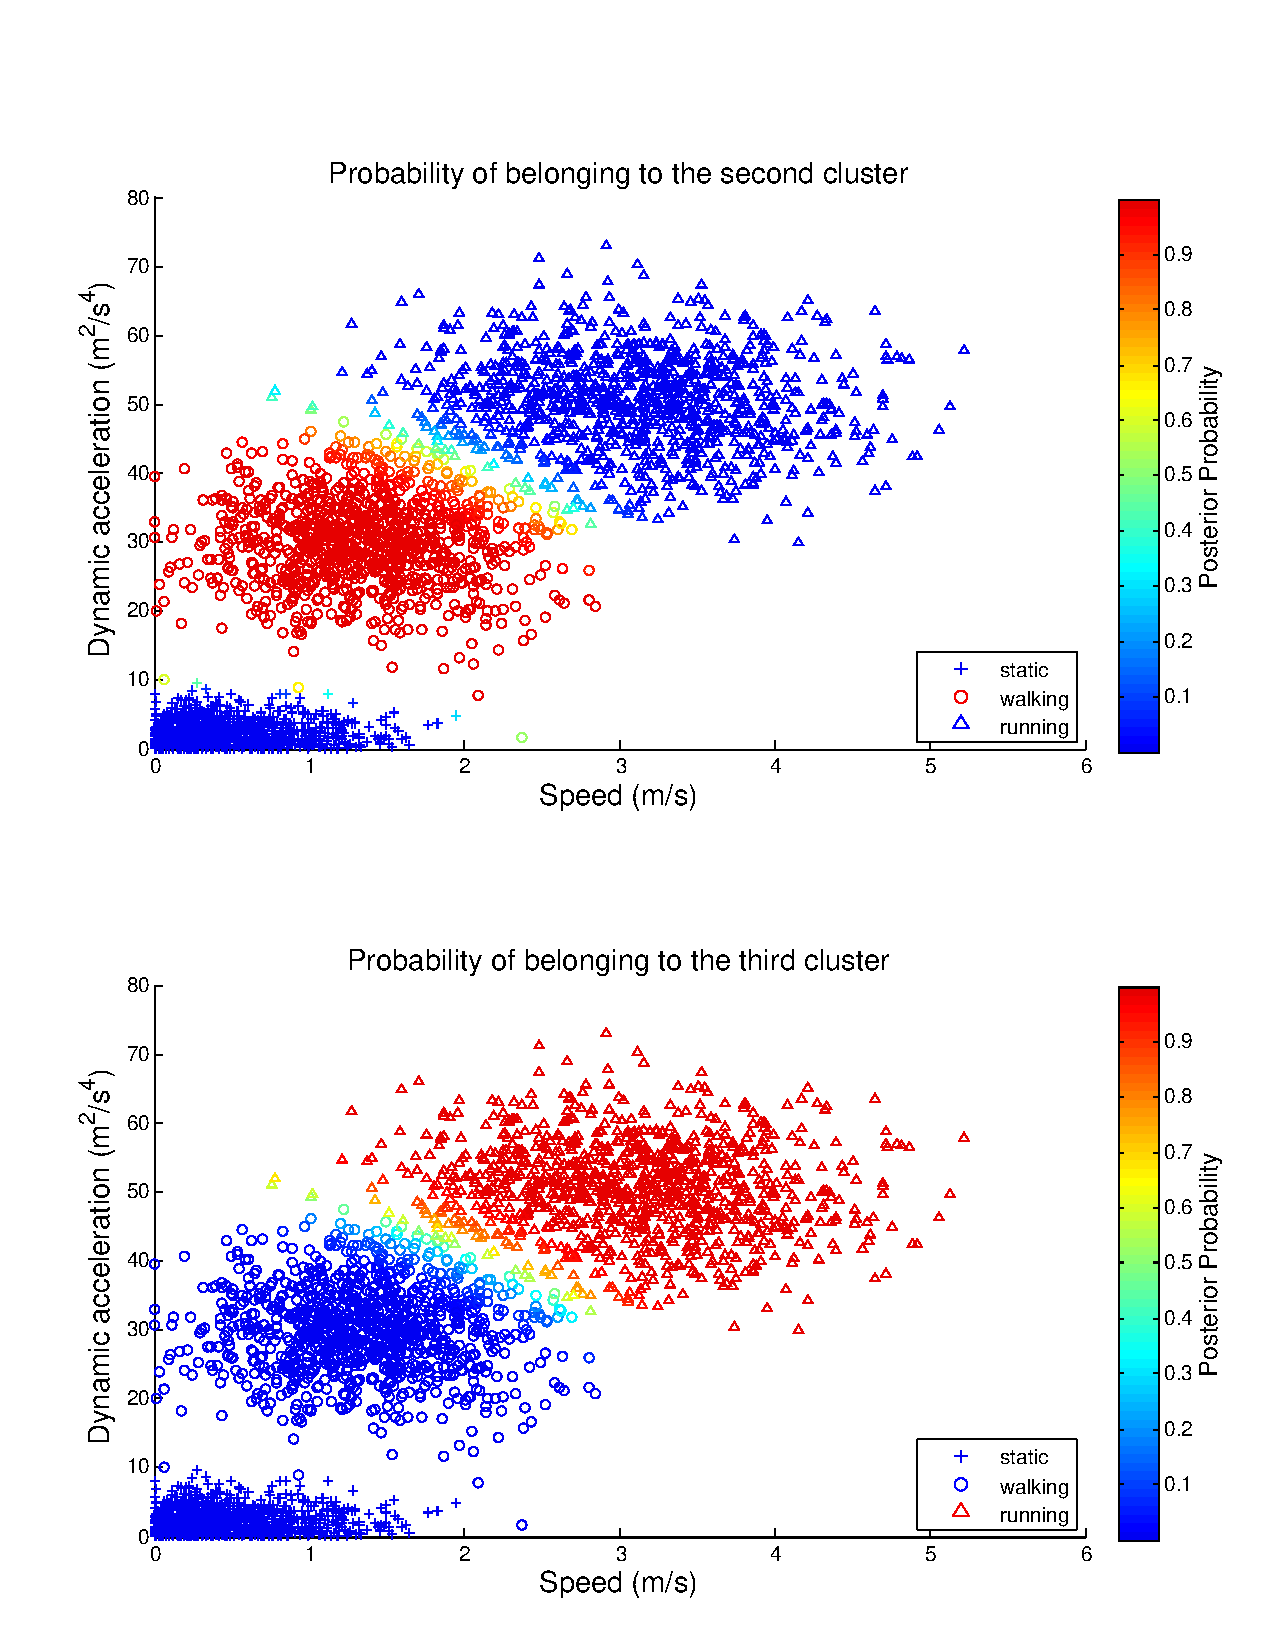
\includegraphics[width=1.0\textwidth]{Images/figChapter3-3}
  \end{center}
  \caption[Further results from unsupervised learning]{These two plots continue the results presented in Figure~\ref{fig:data-from-phone-unsupervised}. The coloring used in the top plot shows the posterior probabilities that the points belong to the second component in a GMM, whereas the bottom plot shows the same for the third component. As in Figure~\ref{fig:data-from-phone-unsupervised}, the data labels are shown strictly for demonstration purposes.}
  \label{fig:data-from-phone-unsupervised2}
\end{figure}
%
%\section{Semi-supervised Learning}
%\label{sec:semi-supervised-learning}

%\section{Conclusions}
%\label{sec:conclusions-ml}

%If the task is formulated in a slightly different way, however, it could be truly considered a machine learning task. We formulate this task as follows:
%
%Let P be a process whose state can be characterised by a value S, which is not directly measurable by any known means. Furthermore, let P produce a set of N-dimensional data X, which can %be measured (e.g. by a set of sensors). Lastly, to keep things simple, let there be a steady-state but unknown relationship F between S and X, such that F(X) = S. 